\documentclass[11pt]{article}
\usepackage[margin=1in]{geometry}
\usepackage{amsmath,amssymb,amsthm}
\usepackage{microtype}
\usepackage{graphicx}
\usepackage{xcolor}
\usepackage{booktabs}
\usepackage{float}
\usepackage{tikz}
\usepackage[numbers,sort&compress]{natbib}
\usepackage{xurl}
\usepackage[colorlinks=true,linkcolor=blue!50!black,citecolor=blue!50!black,urlcolor=blue!50!black]{hyperref}

\emergencystretch=2em
\widowpenalty=10000 \clubpenalty=10000
\makeatletter % a list never starts a page apart from its lead-in
\let\kept@itemize\itemize \def\itemize{\@beginparpenalty\@M\kept@itemize}
\let\kept@enumerate\enumerate \def\enumerate{\@beginparpenalty\@M\kept@enumerate}
\makeatother

\theoremstyle{plain}
\newtheorem{lemma}{Lemma}

\newcommand{\dd}{\mathrm{d}}
\newcommand{\eps}{\varepsilon}
\newcommand{\Hp}{\mathcal H^+}
\newcommand{\pending}[1]{\textcolor{red!60!black}{[Pending #1]}}

\title{Linear radial instability of the Bronnikov--Fabris black universes,\\including the member whose horizon sits at the throat}
\author{Nathan Moinvaziri\thanks{\href{mailto:nathan@nathanm.com}{nathan@nathanm.com}}\\[2pt]
\normalsize\textit{Independent researcher}}
\date{November 2026}

\begin{document}
\maketitle

\begin{abstract}
The black universes of Bronnikov and Fabris are regular black holes held up by a phantom scalar field with a potential.
Beyond the horizon each contains an expanding universe. In units of the throat radius $b$ they are the members $c<0$ of a
one-parameter family. We count their growing spherically symmetric (radial) modes at 20 members, $c=-10$ to $-0.01$. The 19
members with $c\ne-1$ have exactly one each. The growth rate $W$ of that mode runs from $0.0895/b$ at $c=-10$ to $1.1741/b$ at $c=-0.01$,
and tends to the surface gravity $\kappa=2/(\pi b)$ of the horizon as $c\to-1$ from either side. The member $c=-1$, whose
horizon sits at the throat, has no normalizable mode. It has instead a growing solution of rate $\kappa$ carried by the
horizon: there the perturbation of the areal radius is $\delta r=c_1+c_2e^{\kappa v}$, with $v$ the advanced time, and $c_2$
is a free number of regular data on a slice through the horizon. We prove that $c_2$ is gauge invariant on every
non-extremal Killing horizon at an extremum of the areal radius, and that such a horizon needs a metric function that is
not a function of the areal radius alone. Nonlinear double-null evolutions along each member's growing solution give a
lifetime law whose slope is $1/W$ at $c=-0.3$ and $-1.5$ and $1/\kappa$ at $c=-1$, to $2.4\times10^{-4}$. Polar
perturbations with $\ell=1$ and $2$ add no growing mode, and 54 of 55 members with a magnetic field or with the source of the
Simpson--Visser black bounce have a growing radial mode, the exception being the $c=-1$ member. The counts and rates are numerical evidence; the statement on Killing horizons is
proved by hand.
% NEEDS #260: a sentence on what is new, after the literature check.
\end{abstract}

\tableofcontents

\section{Introduction}\label{sec:intro}

Take the member $c=-1$ of the family. Seen from outside it is a black hole of mass $m=2b/(3\pi)$. Its spheres of symmetry
have their smallest area on the horizon itself, at radius $b$, and grow again inside, where the region beyond the horizon
expands toward a de Sitter future~\cite{BF06}. Bronnikov, Konoplya and Zhidenko studied the family under spherically symmetric
perturbations and concluded that ``all configurations under study are unstable under spherically symmetric perturbations,
except for a special class of black universes where the event horizon coincides with the minimum of the area
function''~\cite{BKZ12}. That class is this member. % NEEDS #260
This paper counts the growing modes of the family, and shows that the $c=-1$ member has a growing solution that a count of
normalizable modes does not see. % NEEDS #260

Bronnikov and Fabris constructed the family by choosing the areal radius and the scalar and solving for the
potential~\cite{BF06}; Bronnikov, Dehnen and Melnikov call such regular black holes, with an expanding region beyond the horizon, black
universes~\cite{BMD07}. Bronnikov, Konoplya and
Zhidenko tested their stability by effective potentials and time-domain profiles at several members, and showed the
wormholes of the same family with an anti-de Sitter end unstable~\cite{BKZ12}. Bolokhov, Bronnikov and Skvortsova added a
magnetic field~\cite{BBS12}, and Bronnikov and Walia showed that the Simpson--Visser black bounce~\cite{SV19} is a solution
with a phantom scalar and a magnetic field in nonlinear electrodynamics~\cite{BW22}. The member $c=0$ is the wormhole of
Ellis and Bronnikov~\cite{Ellis1973,Bronnikov1973}, which has one growing radial mode~\cite{GGS2009a}; its polar
perturbations were treated by Azad et al.~\cite{ABCKY23}.

The contributions are:
\begin{itemize}
\item The count and the rates at 20 members: exactly one growing radial mode at each member with $c\ne-1$, with a rate that
  tends to $\kappa$ as $c\to-1$ because the mode becomes a Pöschl--Teller bound state that keeps its shape while it moves
  onto the horizon (Sec.~\ref{sec:results}, Table~\ref{tab:members}, Fig.~\ref{fig:rates}).
\item The $c=-1$ member: a growing solution of rate $\kappa$ whose amplitude $c_2$ is a free number of regular data at the
  horizon, and Lemma~\ref{lem:horizon}, which says why this happens only for a horizon at an extremum of the area
  (Sec.~\ref{sec:cm1}, proof in Appendix~\ref{app:proof}).
\item Nonlinear evolutions whose lifetime slope is $1/W$ at two members and $1/\kappa$ at $c=-1$ (Sec.~\ref{sec:nonlinear}).
\item No growing polar mode with $\ell=1$, $2$, and growing radial modes with two other sources (Secs.~\ref{sec:polar}
  and~\ref{sec:sources}).
\end{itemize}

Status words follow one convention: \emph{proved} (by hand), \emph{checked symbolically} (computer algebra), \emph{numerical
evidence} (a converged computation, no rigorous bound), \emph{conditional} (with the hypothesis named). Every count and rate
in this paper is numerical evidence.

\section{Setting}\label{sec:setting}

\subsection{The family}

We use the conventions of Ref.~\cite{BF06}: signature $(+,-,-,-)$, a scalar $\varphi$ with kinetic sign $\eps$ and potential
$V(\varphi)$, and the field equations
\begin{equation}
R_{\mu\nu}-\eps\,\partial_\mu\varphi\,\partial_\nu\varphi-V g_{\mu\nu}=0,\qquad \eps\,\Box\varphi-V_\varphi=0 .
\end{equation}
A phantom field has $\eps=-1$. For the static metric
\begin{equation}
\dd s^2=A(\rho)\,\dd t^2-\frac{\dd\rho^2}{A(\rho)}-R(\rho)^2\,\dd\Omega^2
\end{equation}
the difference of the $tt$ and $\rho\rho$ equations gives $2R''/R=-\eps\varphi'^2$, so a minimum of the areal radius $R$, a throat, needs
$\eps=-1$. The family of Ref.~\cite{BF06} is
\begin{equation}
R=\sqrt{\rho^2+b^2},\qquad \varphi=\sqrt2\arctan\frac\rho b,\qquad
A=R^2\Big[\frac{c}{b^2}+\frac1{R^2}+\frac{3m}{b^3}\Big(\frac{b\rho}{R^2}+\arctan\frac\rho b\Big)\Big],\label{eq:family}
\end{equation}
with $V(\varphi)$ fixed by these functions. It is flat at $\rho\to+\infty$, with mass $m$, when $2bc=-3\pi m$. We set $b=1$,
so $3m=-2c/\pi$ and $c$ alone labels a member:
\begin{itemize}
\item $c=0$: the Ellis--Bronnikov wormhole, $A=1$, $V=0$;
\item $-1<c<0$: a black universe whose throat $\rho=0$ lies outside the horizon;
\item $c=-1$: the horizon sits at the throat, $\rho_h=0$;
\item $c<-1$: the throat lies beyond the horizon, $\rho_h>0$;
\item $c>0$: wormholes with an anti-de Sitter end~\cite{BKZ12}, not treated here.
\end{itemize}
The horizon $\rho_h$ is the largest zero of $A$, and its surface gravity is $\kappa=A'(\rho_h)/2$. Beyond it, $\rho<\rho_h$,
$A<0$ and $\rho$ is a time: the region is a Kantowski--Sachs cosmology (homogeneous, with spatial sections
$\mathbb R\times S^2$) that expands without end. At $c=-1$, $A'(0)=4/\pi$, so $\kappa=2/\pi=0.636620$, and the mass is
$m=0.21221$.

\subsection{The perturbation equation}

A radial perturbation with time dependence $e^{Wt}$ changes the metric functions and the scalar. We use the gauge
$\delta\varphi=0$, which exists everywhere because $\varphi'=\sqrt2/R^2$ never vanishes, and write $Y=\delta R$ for the
perturbation of the areal radius. The $t\rho$ equation gives the perturbation of $g_{\rho\rho}$, the scalar equation the
perturbation of $g_{tt}$, and the angular equation the master equation
\begin{equation}
Y''=\Big(\frac2\rho-\frac{A'}A\Big)Y'+\Big(\frac1{R^4}-\frac{A'}{A\rho R^2}-\frac2{AR^2}+\frac{W^2}{A^2}\Big)Y .\label{eq:master}
\end{equation}
The $tt$ and $\rho\rho$ equations then hold identically (checked symbolically). With the tortoise coordinate $x$,
$\dd x=\dd\rho/A$, and $u=Y/\rho$, Eq.~\eqref{eq:master} is the Schrödinger form
\begin{equation}
u_{xx}=(\hat V+W^2)\,u,\qquad
\hat V=\frac{2A^2}{\rho^2}-\Big(1+\frac1{R^2}\Big)\frac{AA'}{\rho}+\frac{A^2}{R^4}-\frac{2A}{R^2}.\label{eq:schrodinger}
\end{equation}
Bronnikov, Konoplya and Zhidenko derived this problem in the gauge $\delta R=0$~\cite{BKZ12}. The map
$\delta\varphi=-\varphi'Y/R'$ takes our equation onto theirs, and $\hat V$ equals their effective potential, their
Eqs.~(40) and~(41), with their $\Psi=-\sqrt2\,u$ (checked symbolically, and numerically to $1.1\times10^{-29}$ at 30 digits).
% NEEDS #260: the printed (36)-(38) of [BKZ12] and the printed (8) of [BF06] disagree with the derivation
% (notes/black_universe/README.md, sections 1 and 2); report after the literature check.
The throat $\rho=0$ is a regular singular point of Eq.~\eqref{eq:master} with exponents $0$ and $3$, and both solutions are
analytic there; in Eq.~\eqref{eq:schrodinger} it is the wall $2A^2/\rho^2$.

\subsection{Boundary conditions}\label{sec:bc}

A growing mode is a solution $Y(\rho)e^{Wt}$ with $W>0$ that is regular on the future horizon and decays at infinity. In
the quasinormal conditions of Ref.~\cite{BKZ12} it is the frequency $\omega=iW$.
\begin{itemize}
\item At a horizon with $\rho_h\ne0$ the exponents of $Y$ are $\pm W/A'(\rho_h)$. The regular solution is
  $Y\propto(\rho-\rho_h)^{W/A'(\rho_h)}$, which is $e^{Wv}$ times a smooth function, with $v=t+x$ the advanced time.
\item At infinity $u\propto e^{-Wx}$.
\item The throat needs no condition: $Y$ is continued around $\rho=0$ along a half circle in the complex $\rho$ plane.
\end{itemize}
At $c=-1$ the horizon is the throat. There the exponents of $Y$ are $1\pm W/A_1$, with $A_1=A'(0)=2\kappa$. The count of
Sec.~\ref{sec:results} takes $Y\propto\rho^{1+W/A_1}$, that is $u\to0$, which sets $Y=0$ on the horizon.
Section~\ref{sec:cm1} returns to the other branch.

A root is a sign change of the Wronskian mismatch between the solution regular at the horizon and the one that decays at
infinity, on $W\in[0.01, 8]$ at 60 (resolution R1) and 150 (R2) log-spaced points, refined by Brent's method. R1 and R2
differ in tolerances, start points and outer radius. Their largest relative difference in $W$ is a resolution spread, not a
rigorous bound. Each root's eigenfunction is integrated and its nodes counted.

\section{Results}\label{sec:results}

\subsection{One growing mode}

Table~\ref{tab:members} lists the members. Nineteen of the 20 members have exactly one growing radial mode, and $c=-1$ has
none under the condition $u\to0$. R1 and R2 give the same counts, with rates that agree to $1.2\times10^{-8}$ or better. No
eigenfunction has a node, so each mode is the ground state of its operator.
\begin{table}[t]
\centering
\caption{The 20 members ($b=1$). $\rho_h$ is the horizon, $\kappa$ its surface gravity, $W$ the rate of the one growing radial
mode, $1/W$ its e-folding time, and the last column the relative difference of $W$ between resolutions R1 and R2.
$^a$No normalizable mode; the horizon sector grows at $\kappa$ (Sec.~\ref{sec:cm1}).}
\label{tab:members}
\begin{tabular}{rrrlrrr}
\toprule
$c$ & $\rho_h$ & $\kappa$ & $W$ & $W/\kappa$ & $1/W$ & R1 v R2 \\
\midrule
$-10$ & 4.197082 & 0.116522 & 0.0895350811 & 0.76840 & 11.169 & $1.2\times10^{-10}$ \\
$-3$ & 1.118725 & 0.351374 & 0.2827745372 & 0.80477 & 3.536 & $3.6\times10^{-10}$ \\
$-2$ & 0.621184 & 0.470502 & 0.3984523430 & 0.84687 & 2.510 & $1.3\times10^{-9}$ \\
$-1.5$ & 0.339617 & 0.551682 & 0.4941711675 & 0.89575 & 2.024 & $1.2\times10^{-10}$ \\
$-1.1$ & 0.075763 & 0.620954 & 0.6031905199 & 0.97139 & 1.658 & $2.6\times10^{-10}$ \\
$-1.01$ & 0.007824 & 0.635123 & 0.6331476235 & 0.99689 & 1.579 & $9.3\times10^{-11}$ \\
$-1.001$ & 0.000785 & 0.636471 & 0.6362712254 & 0.99969 & 1.572 & $1.1\times10^{-10}$ \\
$-1.0001$ & 0.000079 & 0.636605 & 0.6365849043 & 0.99997 & 1.571 & $2.3\times10^{-10}$ \\
$-1$ & 0.000000 & 0.636620 & none$^a$ & -- & -- & -- \\
$-0.9999$ & $-0.000079$ & 0.636635 & 0.6366546434 & 1.00003 & 1.571 & $1.2\times10^{-8}$ \\
$-0.999$ & $-0.000786$ & 0.636768 & 0.6369686164 & 1.00031 & 1.570 & $3.0\times10^{-10}$ \\
$-0.99$ & $-0.007884$ & 0.638098 & 0.6401216241 & 1.00317 & 1.562 & $5.4\times10^{-9}$ \\
$-0.95$ & $-0.040055$ & 0.643811 & 0.6544315613 & 1.01650 & 1.528 & $7.9\times10^{-10}$ \\
$-0.9$ & $-0.081826$ & 0.650428 & 0.6730206207 & 1.03473 & 1.486 & $2.8\times10^{-9}$ \\
$-0.7$ & $-0.271920$ & 0.668151 & 0.7558707523 & 1.13129 & 1.323 & $2.5\times10^{-9}$ \\
$-0.5$ & $-0.524073$ & 0.660873 & 0.8541005253 & 1.29238 & 1.171 & $2.4\times10^{-10}$ \\
$-0.3$ & $-0.926754$ & 0.601300 & 0.9700800261 & 1.61331 & 1.031 & $1.8\times10^{-10}$ \\
$-0.2$ & $-1.284188$ & 0.532819 & 1.0354140714 & 1.94327 & 0.966 & $7.9\times10^{-11}$ \\
$-0.1$ & $-2.024885$ & 0.409506 & 1.1059696680 & 2.70074 & 0.904 & $8.7\times10^{-11}$ \\
$-0.01$ & $-7.002156$ & 0.140086 & 1.1741182764 & 8.38142 & 0.852 & $1.9\times10^{-10}$ \\
\bottomrule
\end{tabular}
\end{table}

In plain terms: every member but one has a single way to fall apart, and it is fast. The e-folding time $1/W$ runs from
$0.852\,b$ near the wormhole to $11.169\,b$ at $c=-10$, and $W$ falls monotonically with $-c$. At $c=0$ the same code gives
the Ellis--Bronnikov value $W^2b^2=1.397052434332310$, against $1.39705243433350684$ from an independent quad-double
integration~\cite{Moinvaziri2026c}, a difference of $1.2\times10^{-12}$.

\subsection{The approach to \texorpdfstring{$c=-1$}{c = -1}}\label{sec:limit}

Bronnikov, Konoplya and Zhidenko observed that the growth rate does not decrease as $c$ approaches $-1$~\cite{BKZ12}. The
rates here tend to the surface gravity: $W/\kappa=0.99969$ and $0.99997$ at $c=-1.001$ and $-1.0001$, and $1.00003$ and
$1.00031$ at $c=-0.9999$ and $-0.999$ (Fig.~\ref{fig:rates}).

The reason is a fixed bound state. Write $\rho=\rho_h\,s$ at fixed $s$ and let $\rho_h\to0$. Then $\hat V$, as a function of
$x$, tends to
\begin{equation}
\hat V\to-\frac{A_1^2/2}{\cosh^2(A_1x/2)}\quad(c\to-1^-),\qquad
\hat V\to\frac{A_1^2/2}{\sinh^2(A_1x/2)}\quad(c\to-1^+),
\end{equation}
with $A_1=A'(\rho_h)$ (checked symbolically). The first is the $\ell=1$ Pöschl--Teller well~\cite{PT1933}, with the bound
state $u=1/\cosh(A_1x/2)$ at $W=A_1/2=\kappa$. The second contains the throat's wall, and $u=1/\sinh(A_1x/2)$ gives a regular
$Y=\rho u$ at the same $W$. The members $c=-1.0001$ and $-0.9999$ follow these limits to $1.5\times10^{-3}$ and
$1.3\times10^{-3}$ (relative). As $\rho_h\to0$ the well keeps its shape and moves toward $x\to-\infty$, like
$(1/A_1)\ln|\rho_h|$, so the bound state keeps $W=\kappa$. At $c=-1$ exactly there is no well at finite $x$: the wall and the
horizon cancel, $\hat V\to0$ at the horizon, and there is no bound state. So the count is 0 at one point and 1 at points
arbitrarily close to it, with a rate near $\kappa$, not near zero.

\pending{\#262: $\dd(W/\kappa)/\dd c$ at $c=-1$ from either side, and its closed form, from the $c=-1$ solution of
Sec.~\ref{sec:cm1}.}

\begin{figure}[t]
\centering
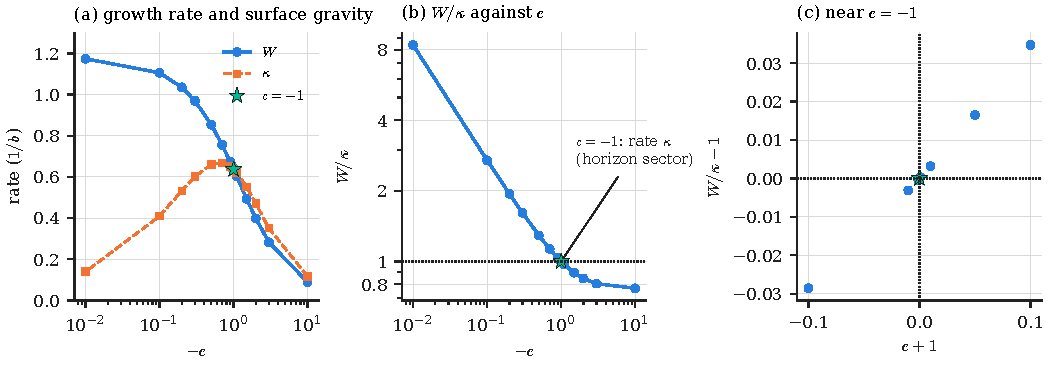
\includegraphics[width=\textwidth]{fig_rates.pdf}
\caption{(a) The rate $W$ of the one growing radial mode and the surface gravity $\kappa$ against $-c$ ($b=1$). (b) $W/\kappa$.
(c) $W/\kappa-1$ near $c=-1$. The star at $c=-1$ is the rate of the horizon sector from the linear double-null solver of
Sec.~\ref{sec:cm1}, $0.636627$ against $\kappa=0.636620$; at $c=-1$ the count of normalizable modes is zero.}
\label{fig:rates}
\end{figure}

\subsection{Second methods}

A Chebyshev collocation of Eq.~\eqref{eq:schrodinger} (for $c\le-1$) or Eq.~\eqref{eq:master} (for $c>-1$) as a matrix
eigenvalue problem shares the background and the coefficients with the shooting code and nothing of the boundary
conditions, the throat crossing or the root finding. At $N=401$ and $801$ points it gives the same counts at all 20 members,
40 of 40, and no complex eigenvalue. At $N=801$ its rates agree with the shooting to $4.55\times10^{-7}$ for $c\le-1$; for the
throat members, where it converges slowly, they agree to $4.54\times10^{-3}$. For the nine members with $c\le-1$ a finite-difference
eigenvalue code written separately for review gives the same counts, with $W$ equal to the shooting to $2.4\times10^{-10}$,
and none at $c=-1$. A recount of seven members on the wider range $W\in[10^{-5},8]$, with a range-free Sturm count where
$c\le-1$, gives the same counts, with $W$ equal to Table~\ref{tab:members} to $2.8\times10^{-9}$ (R1) and $3.6\times10^{-10}$
(R2).

\subsection{Polar perturbations}\label{sec:polar}

For $\ell\ge2$ we use the Regge--Wheeler gauge, which is complete there and has no singular point at the throat. For $\ell=1$
we use the gauge with $h_{t\rho}=0$ of Ref.~\cite{ABCKY23} and remove its residual gauge solution by a determinant. At the 20
members and at the wormhole $c=0$, polar $\ell=1$ and $\ell=2$ have no growing mode with real $W\in[0.01, 8]$: 84 runs, with
determinants that agree between R1 and R2 to $5.1\times10^{-9}$ (numerical evidence). At $c=0$ the absence is also
checked symbolically: the master potentials are $\ell(\ell+1)/R^2-3/R^4$ for $\ell\ge2$ and $1/R^4$ for $\ell=1$, both positive.
Complex $W$ is not searched. As a planted case the same code gives the polar quasinormal modes of the wormhole at $\ell=2$,
3, 4 as $1.737692-0.305138i$, $2.952415-0.409984i$ and $4.076253-0.449105i$, against $1.74-0.305i$, $2.95-0.410i$ and
$4.08-0.449i$ in Table~1 of Ref.~\cite{ABCKY23}.

\subsection{Other sources}\label{sec:sources}

The same method applies to two sources that add a field. S is the Simpson--Visser metric $A=1-2m/R$ with the phantom scalar
and nonlinear magnetic field of Ref.~\cite{BW22}, at zero charge. B is the magnetic black universe of Ref.~\cite{BBS12}, with
charge $q$. A magnetic field adds no radial degree of freedom (checked symbolically): the master equation keeps its form, with
the extra term $-RA\Lambda_R$ in $\hat V$, where $\Lambda$ is the field's energy density. Table~\ref{tab:sources}
gives the counts, and 54 of 55 members have a growing radial mode. The exception is $q=0$ on the slice B2, which is the $c=-1$
member. B2 keeps the horizon at the throat as $q$ grows, and every $q>0$ on it has one growing mode, with
$W=0.0037625403$ at $q=0.1$ rising to $W=0.1675848842$ at $q=0.81$. A Maxwell field therefore does not stabilize the
$c=-1$ member. The counts with these sources use the condition $u\to0$ at the horizon; whether the horizon sector of
Sec.~\ref{sec:cm1} exists on B2 was not computed.
\nopagebreak
\begin{table}[H]
\centering
\caption{Radial modes with a second source (numerical evidence). A member counts as unstable if it has a real growing mode
or a complex-conjugate pair with $\mathrm{Re}\,W>0$. B1 and B3 have fixed mass $m$.}
\label{tab:sources}
\begin{tabular}{llrr}
\toprule
slice & members & tested & growing \\
\midrule
S & Simpson--Visser, $m=M/a$ from 0 to 10 & 16 & 16 \\
B1 & $m=2/\pi$ ($c=-3$ at $q=0$), $q$ from 0 to 0.775 & 12 & 12 \\
B2 & horizon at the throat, $q$ from 0 to 0.81 & 12 & 11 \\
B3 & $m=0.2/\pi$ ($c=-0.3$ at $q=0$), $q$ from 0 to 0.24 & 11 & 11 \\
P & zero charge, $c=-10$, $-1.1$, $-0.9$, $-0.01$ & 4 & 4 \\
\midrule
all & & 55 & 54 \\
\bottomrule
\end{tabular}
\end{table}

Three members have a complex pair, two of them without a real mode, and several have a second, weak real mode; the notes list
them. The results hold for these two sources only: the same metric may have different stability with another
source~\cite{BW22}.

\section{The member whose horizon sits at the throat}\label{sec:cm1}

\subsection{Two branches at the horizon}\label{sec:branches}

At $c=-1$ the exponents of $Y$ at $\rho=0$ are $1\pm W/(2\kappa)$. Near the horizon $\rho\propto e^{2\kappa x}(1+O(\rho))$, so
a branch $\rho^s e^{Wt}$ equals $e^{Wv}$ times $\rho^{s-W/(2\kappa)}$ times an analytic function. The branch $s=1+W/(2\kappa)$
is the one counted above; it vanishes on the horizon. The branch $s=1-W/(2\kappa)$ is $e^{Wv}\rho^{1-W/\kappa}$ times an
analytic function, which is smooth on the future horizon only when $W=\kappa$. There the Frobenius recursion could still
produce a logarithm, with coefficient $\pi w(1-w)/8$, $w=W/\kappa$, which vanishes at $w=1$ (checked symbolically). So at
$W=\kappa$ there is a solution $Y\propto e^{\kappa v}$, smooth and nonzero on the future horizon. At $c\ne-1$ the exponents at
$W=\kappa$ are $\pm1/2$ and the branch $-1/2$ diverges: the regular solution growing at $\kappa$ exists at $c=-1$ alone
(checked symbolically, by hand and in SymPy, in the review). It is not a normalizable mode: on a slice of constant $t$ it
grows toward large $\rho$, and $u=Y/\rho$ diverges at the horizon. The count of Sec.~\ref{sec:results} therefore cannot see
it. Whether it is excited by physical data is the question of the rest of this section.

\subsection{The linear double-null evolution}\label{sec:dn}

We linearized the three evolution equations of a double-null code with the potential about the member, in a null chart that
crosses the future horizon into the interior, and evolved data given on two null rays. The scheme is second order: exact
pure-gauge solutions are reproduced with errors that fall by 4.00 per halving of the step, and the linearized constraints
fall by 3.99 to 4.00 per halving. It reproduces the rates of Table~\ref{tab:members} to $9.2\times10^{-5}$ at $c=-1.5$, $2.0\times10^{-7}$
at $c=-0.3$, $1.3\times10^{-5}$ at $c=-1.01$ and $1.1\times10^{-5}$ at $c=-0.99$. The data are a Gaussian pulse of the scalar
on one ray or both, or a constant of $\delta r$ or of one of its null derivatives at the corner of the two rays.
Table~\ref{tab:classes} gives the rate of $Y$ at the static observer's position $x=0$.
\nopagebreak
\begin{table}[H]
\centering
\caption{The $c=-1$ member in the linear double-null solver ($\kappa=0.636620$). $Y_h(0)$ is $Y$ where the data ray that
crosses the horizon meets it, and the rates are those of $Y(x=0)$ over $t\in[16,20]$, Richardson of two steps. The last column is the
master equation~\eqref{eq:schrodinger} in characteristic form, fed $u$ of the same data on the two rays.}
\label{tab:classes}
\begin{tabular}{llrrr}
\toprule
class & data & $Y_h(0)$ & rate & rate, Eq.~\eqref{eq:schrodinger} \\
\midrule
R & pulse on the exterior ray (an ingoing wave) & 0 & 0.01154 & $-0.00859$ \\
L & pulse on the ray that crosses the horizon & $-1.474\times10^{-4}$ & 0.63661 & 0.63661 \\
G & both pulses & $-1.474\times10^{-4}$ & 0.63663 & 0.63663 \\
A0 & corner $\delta r$ & $1.262\times10^{-3}$ & 0.63662 & 0.63662 \\
A1R & corner $\partial_p\delta r$ & 0 & 0.63662 & 0.00472 \\
A1L & corner $\partial_\sigma\delta r$ & $2.467\times10^{-3}$ & 0.63660 & 0.63662 \\
\bottomrule
\end{tabular}
\end{table}

Every class but R grows at $\kappa$; data G give $0.636627$ against $\kappa=0.636620$. Class R, a wave
sent in on an unperturbed horizon, does not grow; its small rate is the truncation seed, which falls as $h^2$. The growth is
carried by the horizon values of $Y$. On the horizon the null constraint reduces to $\partial^2_V\delta r=0$ (Lemma~\ref{lem:horizon}), so
$Y_h=c_1+c_2e^{\kappa v}$: for three pulses the late exponent of $Y_h$ in the null time $p$ equals $\sqrt2\kappa=0.900316$
to $7.4\times10^{-8}$. Combining the three so that $c_1=c_2=0$ reduces $|Y(x=0)|$ at $t=14$ by $2.44\times10^4$, and the
combination decays, at rate $-0.1768$. The same operation at $c=-1.5$ reduces it only by $40.3$ and leaves the rate at $0.4777$,
near $W=0.4942$: the horizon sector is specific to $c=-1$. Near the horizon the late profile of $Y$ goes as $\rho$ to the
power $0.4995$, the branch $1/2$ of Sec.~\ref{sec:branches}, and not $3/2$.

The master equation in characteristic form reproduces the double-null $Y$ for the pulse classes to $8.8\times10^{-4}$ of its
running maximum, and it too grows at $\kappa$ when fed the same data. So the equation is right, and the difference with the
count lies only in the condition at the horizon.

\subsection{The growing amplitude is free in Cauchy data}\label{sec:cauchy}

To ask whether $c_2$ belongs to physical initial data we need a chart that contains a spacelike slice through the horizon.
Let $\Pi=e^{2\kappa x}$ and $V=e^{\kappa v}$, $U=-\Pi/V$. The member in these Kruskal coordinates is
\begin{equation}
\dd s^2=2e^{-F}\dd V\,\dd U-r^2\dd\Omega^2,\qquad r=R(\rho(\Pi)),\qquad e^{-F}=\frac{1}{2\kappa^2\Pi}A ,
\end{equation}
with $\rho(\Pi)$ analytic through $\Pi=0$. The chart contains the future horizon $\Hp$ ($U=0$), the bifurcation sphere $S$
($U=V=0$) and the interior ($\Pi<0$, where $\rho<0$) up to $\rho\to-\infty$ (Fig.~\ref{fig:kruskal}). The
quantity $Y=\delta r-(\rho R/\sqrt2)\,\delta\varphi$ is invariant under every linear diffeomorphism and equals $\delta R$ in the
gauge $\delta\varphi=0$; on $\Hp$ at $c=-1$, $\rho=0$ and $Y=\delta r$.
\begin{itemize}
\item \emph{The law.} On $\Hp$ the linearized $VV$ constraint is $\partial_V^2\delta r=0$, so $\delta r=c_1+c_2V$ along the
  whole horizon, from $S$ outward (Lemma~\ref{lem:horizon}).
\item \emph{The functional.} For the slice $V+U=\mathrm{const}$ crossing $\Hp$, with tangent $T=\partial_V-\partial_U$ and normal
  $N=\partial_V+\partial_U$, $c_2=\tfrac12(\partial_T\delta r+\partial_N\delta r)$ at the crossing: a combination of the slice
  values and their normal derivative.
\item \emph{Free.} The linearized constraints propagate, $\partial_U\delta C_{VV}=-(r_U/r)\,\delta C_{VV}$ and
  $\partial_V\delta C_{UU}=-(r_V/r)\,\delta C_{UU}$, for any background that solves the field equations (checked
  symbolically). They restrict second derivatives only, so the first-order data at a point of $\Hp$, $c_2$ among them, are
  free.
\item \emph{Gauge invariant.} At the area minimum $r_U=r_V=0$ on $\Hp$, so no shift of the horizon's position changes
  $\delta r$ there (Lemma~\ref{lem:horizon}).
\item \emph{Regular.} The growing solution is $Y=c_2VG(\Pi)$, with $G$ analytic in $\Pi$: smooth across $S$ and into the
  interior. A formal series at $S$ shows that the smooth solutions contain the two branches $Y\propto V$ and $Y\propto U$ and
  otherwise only solutions with smooth $u$ (checked symbolically); the series at $W=\kappa$ has no logarithm.
\end{itemize}

A second solver works in this chart, through $S$ and the interior, and evolves data on the rays $V=-0.05$ and $U=-2$.
Table~\ref{tab:c2} gives $c_1=Y(S)$ and $c_2$ for the data classes, by a fit of the horizon values; the slice functional at
the crossings $V=0$, $0.5$ and $1$ gives the same $c_2$ to $6.8\times10^{-8}$. On the solutions of Sec.~\ref{sec:dn} the slice
functional equals the horizon fit to $3.5\times10^{-10}$ after Richardson extrapolation. Twenty random smooth data (corner
constants and scalar pulses on both rays) have $|c_2|$ from $3.40\times10^{-4}$ to $2.10\times10^{-2}$, median
$7.74\times10^{-3}$; none has $c_2=0$.
\nopagebreak
\begin{table}[H]
\centering
\caption{$c_1=Y(S)$ and $c_2=\partial_V\delta r$ on $\Hp$ for data of amplitude $10^{-3}$ at $c=-1$, Kruskal chart,
Richardson of $h=0.0025$ and $0.00125$. Class L has no data on the exterior ray; class R has data only there.}
\label{tab:c2}
\begin{tabular}{llrr}
\toprule
class & data & $c_1$ & $c_2$ \\
\midrule
L & scalar pulse on $V=-0.05$, centred on $U=0$ & $-9.3\times10^{-13}$ & $-9.610862\times10^{-4}$ \\
G & L and a pulse on $U=-2$ & $-4.8\times10^{-12}$ & $-9.610862\times10^{-4}$ \\
A0 & corner $\delta r$ & $1.658047\times10^{-3}$ & $1.227043\times10^{-2}$ \\
A1R & corner $\partial_V\delta r$ & $5.236768\times10^{-5}$ & $1.047354\times10^{-3}$ \\
A1L & corner $\partial_U\delta r$ & $2.094707\times10^{-3}$ & $1.007157\times10^{-2}$ \\
R & pulse on $U=-2$ only & $-3.9\times10^{-12}$ & $5\times10^{-13}$ (seed) \\
\bottomrule
\end{tabular}
\end{table}

Class L puts a scalar pulse across the horizon and nothing on the exterior ray, and has $c_2=-9.610862\times10^{-4}$. A
transport of the transverse derivatives along the data ray $V=-0.05$, written for review and sharing no code with either
solver, gives $c_2=-9.61086221626\times10^{-4}$, which agrees to $2.3\times10^{-8}$. Class R gives $c_2=0$ up to a seed of
$1.8\times10^{-9}$ at $h=0.00125$ that falls by 4 per halving. As a planted case, pure-gauge data at $c=-1.5$, where $c_2$ is
gauge and known in closed form ($-1.12925016\times10^{-2}$), are recovered to $3.6\times10^{-9}$ on exact data and
$1.4\times10^{-8}$ on the evolved solution.

In plain terms: the linear problem about the $c=-1$ member has one growing direction of rate $\kappa$, like the other 19
members, but it lives on the horizon. Its amplitude $c_2$ is one number, set by the data at and before the horizon crossing.
Data with $c_2=0$, among them all data supported away from the crossing, do not grow at $\kappa$; data with $c_2\ne0$ do, and
generic data have $c_2\ne0$. The count of normalizable modes is the count for $c_1=c_2=0$. These statements rest on the
solvers' domain, which covers a bounded neighbourhood of $S$ and of the horizon crossing; a compactly supported datum on a full slice to spatial
infinity with zero change of the mass has not been built.

\pending{\#258: a compactly supported datum on a full slice to spatial infinity, its constraint solution, and its $c_2$.}

\pending{\#262: the closed form of the $c=-1$ solution $Y=VG(\Pi)$.}
\nopagebreak
\begin{figure}[H]
\centering
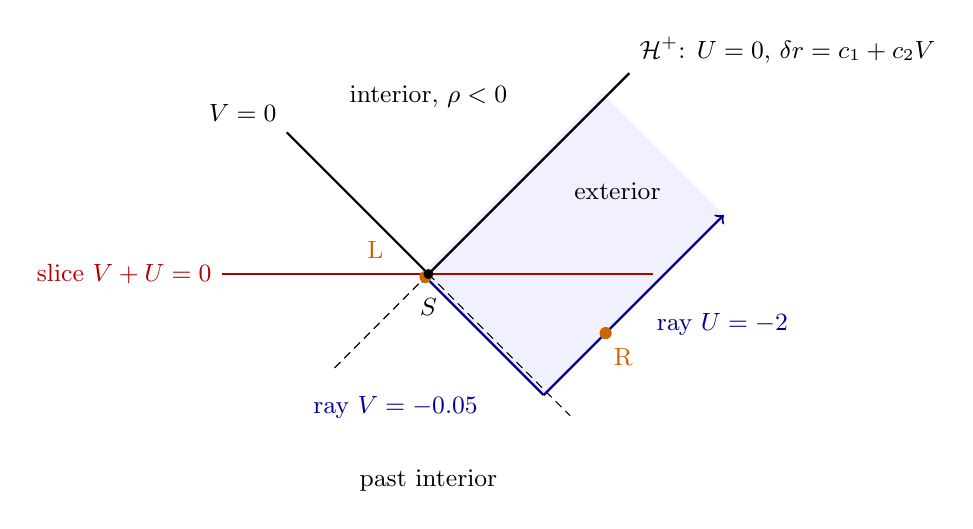
\begin{tikzpicture}[x={(0.75cm,0.75cm)}, y={(-0.75cm,0.75cm)}, font=\small]
\fill[blue!6] (-0.05,-2) -- (3,-2) -- (3,0.06) -- (-0.05,0.06) -- cycle;
\draw[thick] (0,0) -- (3.4,0) node[above right] {$\Hp$: $U=0$, $\delta r=c_1+c_2V$};
\draw[thick] (0,0) -- (0,2.4) node[above left] {$V=0$};
\draw[densely dashed] (0,0) -- (0,-2.4);
\draw[densely dashed] (0,0) -- (-1.6,0);
\draw[red!70!black, thick] (1.9,-1.9) -- (-1.75,1.75) node[left] {slice $V+U=0$};
\draw[->, thick, blue!60!black] (-0.05,-2) -- (3,-2);
\node[blue!60!black, anchor=north west] at (1.6,-2.1) {ray $U=-2$};
\draw[->, thick, blue!60!black] (-0.05,-2) -- (-0.05,0.06);
\node[blue!60!black, anchor=north east] at (-0.45,-1.45) {ray $V=-0.05$};
\fill[orange!80!black] (-0.05,0) circle (2.2pt);
\node[orange!80!black, anchor=east] at (-0.1,0.5) {L};
\fill[orange!80!black] (1,-2) circle (2.2pt);
\node[orange!80!black, anchor=north] at (1.1,-2.2) {R};
\fill (0,0) circle (1.8pt);
\node[anchor=north] at (-0.12,-0.12) {$S$};
\node at (1.5,1.5) {interior, $\rho<0$};
\node at (2.3,-0.9) {exterior};
\node at (-1.75,-1.75) {past interior};
\end{tikzpicture}
\caption{Kruskal chart of the $c=-1$ member (time upward; $V$ increases to the upper right, $U$ to the upper left). The
shaded rectangle is the second solver's domain, with data on the two rays. Class L puts a pulse where the ray $V=-0.05$
crosses the horizon's line, class R a pulse on the exterior ray. The slice $V+U=0$ passes through the bifurcation sphere $S$.}
\label{fig:kruskal}
\end{figure}

\subsection{Why only a horizon at an extremum of the area}\label{sec:lemma}

The horizon law and the gauge invariance of $c_2$ hold beyond this family. Consider a static spherically symmetric solution
in $D=n+2$ dimensions, $n\ge2$, of Einstein gravity with a scalar of either kinetic sign and any potential, with a bifurcate
Killing horizon of surface gravity $\kappa>0$. In Kruskal coordinates the metric is $\pm(2e^{-F}\dd V\dd U-r^2\dd\Omega_n^2)$,
the Killing field is $\kappa(V\partial_V-U\partial_U)$, and $r$, $F$, $\varphi$ depend on $(V,U)$ only through $\Pi=-VU$. Write
$r=R(\rho(\Pi))$ with $\rho$ the radial coordinate of the static form, and $\rho'(0)=\dd\rho/\dd\Pi$ at $\Pi=0$, finite and
nonzero. A perturbation $(\delta r,\delta F,\delta\varphi)$ keeps the double-null form.

\begin{lemma}\label{lem:horizon}
For every linear perturbation that solves the linearized field equations:
\begin{enumerate}
\item On $\Hp$, $\partial_V^2\delta r=0$, so $\delta r=c_1+c_2V$ along the whole line $U=0$.
\item Under a linear diffeomorphism $\xi$, $\partial_V(\mathcal L_\xi r)=-R'(\rho_h)\,\rho'(0)\,\partial_V(V\xi^U)$ on $U=0$. If
  $R'(\rho_h)=0$, $c_1$ and $c_2$ are the same in every gauge. If $R'(\rho_h)\ne0$, the shift $U\to U+\eta(U)$ changes $c_2$
  by $-\eta(0)R'(\rho_h)\rho'(0)$, and $c_2$ is pure gauge.
\item If $R'(\rho_h)=0$, the area of the horizon's cross-sections changes by $\Omega_n n r_h^{n-1}(c_1+c_2e^{\kappa v})$ to
  first order. With $c_2\ne0$ the change grows at the surface-gravity rate.
\item If $A=f(R(\rho))$ with $f$ differentiable, then $R'(\rho_h)=0$ forces $A'(\rho_h)=0$, that is $\kappa=0$. A non-extremal
  horizon at an extremum of the areal radius needs a metric function $A$ that is not a function of the areal radius alone.
\end{enumerate}
\end{lemma}

\noindent\emph{Status:} proved by hand; the algebra of each step is checked symbolically. The proof is in
Appendix~\ref{app:proof}.

In plain terms: the background is constant along the horizon's generators, so the null constraint there sees only the
perturbation's own second derivative, and $\delta r$ is linear in $V=e^{\kappa v}$. On an ordinary horizon the linear part is
a relabeling of which null surface is the horizon. At an extremum of the area that relabeling does not change $r$, so the
linear part is physical: the horizon's area grows at the rate $\kappa$. In Schwarzschild, Reissner--Nordström or any metric
with $A$ a function of the areal radius, a horizon at an extremum of the area would have to be extremal. The proof uses the matter only
through the linearized $T_{VV}$ on $\Hp$, which vanishes for the scalar and for any matter whose $T_{VV}$ vanishes on the
background horizon, such as a radial Maxwell field.
\nopagebreak
\begin{table}[H]
\centering
\caption{Lemma~\ref{lem:horizon} applied ($b=1$, $2M=1$ for Schwarzschild).}
\label{tab:lemma}
\begin{tabular}{lrrl}
\toprule
spacetime & $R'(\rho_h)$ & $\kappa$ & $c_2$ \\
\midrule
black universe, $c=-1$ & 0 & $2/\pi$ & invariant, free in data (Sec.~\ref{sec:cauchy}) \\
black universe, $c=-1.5$ & 0.321578 & 0.5516816788 & pure gauge \\
Schwarzschild & 1 & 0.5 & pure gauge \\
Simpson--Visser, $a=2m$ & 0 & 0 & extremal; outside the lemma \\
\bottomrule
\end{tabular}
\end{table}

Of the 20 members of Table~\ref{tab:members}, only $c=-1$ puts the horizon at the throat. On the slice B2 of
Sec.~\ref{sec:sources} the horizon stays at the throat, $\kappa>0$, and the magnetic field has $T_{VV}=0$, so the hypotheses of
items 1 to 3 hold there (by the paragraph on matter in Appendix~\ref{app:proof}); whether $c_2$ is free on B2 was not computed.

\section{Nonlinear evolutions}\label{sec:nonlinear}

A double-null code for the Einstein--phantom equations with the potential evolves the member plus $A$ times its growing
solution, with data on two null rays through a point at $\rho=0$ ($c=-0.3$) or $\rho=1$ ($c=-1.5$, $-1$). The code's
evolution equations equal an independent derivation from a brute-force Ricci tensor to $1.1\times10^{-15}$, and the static
members stay static to second order in the step $h$. The time is the Killing time of the static observer on the diagonal. The
lifetime $T$ is the first time at which $|Y|$ on the diagonal reaches $2\times10^{-5}$, and the outcome is the sign of $Y$
there. A bisection in $A$ finds the threshold $A_*$. Near it a static critical solution with one growing mode predicts
\begin{equation}
T=s\ln\frac1{|A-A_*|}+\mathrm{const},\qquad s=\frac1W,\label{eq:lifetime}
\end{equation}
the lifetime law of type I critical phenomena~\cite{GMG2007}. Each slope is fitted on $|A-A_*|\in[10^{-7},10^{-5}]$, 9
points per side, with one slope for both sides. Three error bars are reported, and they are different things: the
ordinary-least-squares standard error (statistical), the fit spread (the envelope of $s\pm2$ standard errors over 15 fits
with other windows and sides), and the difference between the two finest steps.
\nopagebreak
\begin{table}[H]
\centering
\caption{Lifetime slope $s\pm$ standard error at the two finest steps $h$, against the reference $1/W$ ($c=-0.3$,
$-1.5$) or $1/\kappa$ ($c=-1$), with the relative difference and the fit spread.}
\label{tab:slopes}
\begin{tabular}{rllllr}
\toprule
$c$ & $h$ & $s$ & reference & relative & fit spread \\
\midrule
$-0.3$ & 0.005 & $1.03122\pm0.00178$ & 1.03084 & $+3.6\times10^{-4}$ & [1.02099, 1.04029] \\
$-0.3$ & 0.0025 & $1.03101\pm0.00043$ & 1.03084 & $+1.6\times10^{-4}$ & [1.02764, 1.03369] \\
$-1.5$ & 0.005 & $2.02528\pm0.00706$ & 2.02359 & $+8.3\times10^{-4}$ & [1.94590, 2.11056] \\
$-1.5$ & 0.0025 & $2.02338\pm0.00291$ & 2.02359 & $-1.0\times10^{-4}$ & [1.99256, 2.05635] \\
$-1$ & 0.005 & $1.57170\pm0.00218$ & 1.57080 & $+5.8\times10^{-4}$ & [1.55983, 1.58392] \\
$-1$ & 0.0025 & $1.57042\pm0.00045$ & 1.57080 & $-2.4\times10^{-4}$ & [1.56589, 1.57250] \\
\bottomrule
\end{tabular}
\end{table}

At $c=-0.3$ and $-1.5$ the slope equals $1/W$ within two standard errors at both steps, $1/W$ lies inside each fit spread,
and the difference falls with $h$ (Fig.~\ref{fig:slopes}). The thresholds $A_*$ converge at second order in $h$, with orders
2.037, 2.016, 2.005 ($c=-0.3$), 2.019, 1.990, 1.971 ($c=-1.5$) and 2.035, 2.013, 2.003 ($c=-1$), to $A_*=0$: the threshold of
a family through the static member is the member. On the collapse side every member forms a trapped and an anti-trapped region
in the same run. On the other side $c=-0.3$ forms an anti-trapped region and no trapped one, while at $c=-1.5$ and $-1$ the
trapped-surface finders stay silent until a distant anti-trapped cell, at $t=60.2$ ($c=-1.5$) and $t=50.9$ ($c=-1$) at the
earliest.
\nopagebreak
\begin{figure}[H]
\centering
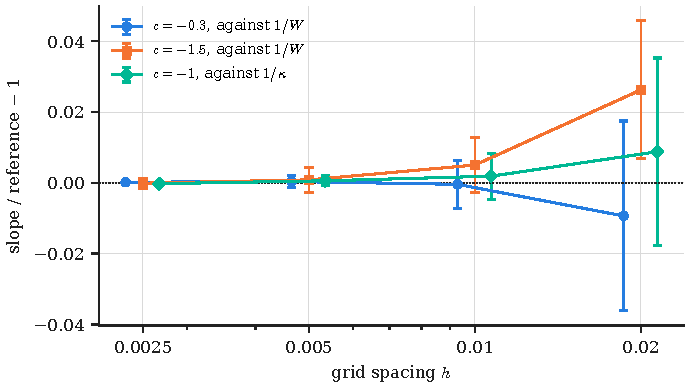
\includegraphics[width=0.66\textwidth]{fig_slopes.pdf}
\caption{Lifetime slope relative to its reference against the step $h$, with the standard error as the bar.}
\label{fig:slopes}
\end{figure}

At $c=-1$ the slope is $1/\kappa$, although the count of Sec.~\ref{sec:results} is zero there. The family member plus $A$
times the code's own growing solution lies in the horizon sector: the code's truncation error seeds $c_2$ at order $h^2$, as
the linear solver's $Y_h$ for class R and the nonlinear code's drift both fall by 4.00, 4.00 and 3.97, 4.01 per halving of
$h$. The nonlinear code reproduces the linear solver's response to the same data to $2.3\times10^{-3}$ until its own drift
reaches $5\times10^{-4}$. A one-dimensional evolution of Eq.~\eqref{eq:schrodinger} with $u\to0$ at the horizon decays at
$c=-1$, at the rate $-0.0370$. So the nonlinear code at $c=-1$ sees the growing direction of Sec.~\ref{sec:cm1}.

These runs test the growth rate in a nonlinear code along a family through the static member. They do not show that generic
data approach the member. A one-sided pulse, a second family, gives the same slope at $c=-0.3$ ($1.03494$ against
$1.03122$) but not at $c=-1.5$ ($1.15004$ against $2.02528$), where the first trapped cell lags the departure from the member by
a delay that depends on $A$.

\section{Consequences and limits}\label{sec:limits}

\begin{itemize}
\item \emph{The family.} Each of the 20 members tested grows: one normalizable mode at each $c\ne-1$, and at $c=-1$ one
  growing direction of rate $\kappa$ on the horizon. In the linear problem the $c=-1$ member grows at $\kappa$ unless
  $c_2=0$, a single condition on the data at the horizon crossing. Between the 20 values of $c$ nothing is computed.
\item \emph{Prior work.} Ref.~\cite{BKZ12} concludes that the black universes ``are shown to be stable only in the special
  case where the horizon coincides with the minimum of the area function $R(r)$ (the parameters: $c=-1$, $b=3\pi m/2$)''.
  For that member this work finds the growing direction of Sec.~\ref{sec:cauchy}, excited by regular data with $c_2\ne0$, and no
  growth for data with $c_2=0$, which include waves sent in on an unperturbed horizon. % NEEDS #260
\item \emph{The mechanism.} Lemma~\ref{lem:horizon} is general: any non-extremal Killing horizon at an extremum of the
  areal radius carries a gauge-invariant $c_2$. Which other known solutions have such a horizon is not examined here.
  % NEEDS #260: the literature search for other horizons at an area extremum is part of #260.
\item \emph{What the rates are.} Counts and rates are numerical evidence: a sign-change search on $W\in[0.01, 8]$ with
  node, spectral and Sturm guards, no argument-principle count and no rigorous bound. The error bars are resolution spreads,
  Richardson differences, standard errors and fit spreads, each named where it is quoted.
\item \emph{Open.}
  \begin{itemize}
  \item A compactly supported datum on a full slice to spatial infinity at $c=-1$ (\#258).
  \item The closed form of the $c=-1$ solution and $\dd W/\dd c$ at $c=-1$ (\#262).
  \item A count with the horizon-regular condition at every member and with the second sources, including B2 (\#249); the
    static sector $c_1$ (\#259).
  \item The nonlinear fate of data with $c_2=0$ and with $c_2\ne0$ at $c=-1$, and the end state on the side without a
    trapped region.
  \item Complex $W$ for the polar systems, $\ell\ge3$, the interior region, and formation by collapse.
  \end{itemize}
\end{itemize}

\section{Computations}\label{sec:computations}

Each result was computed by one code and checked by at least one other that shares as little as possible with it. What the
two share is stated. Each check was broken on purpose by a named mutation (a sign, a coefficient, a dropped term) and seen to
fail.
\begin{itemize}
\item \emph{Background and equations.} The closed forms~\eqref{eq:family} satisfy the field equations with residual 0 in
  SymPy and $9.2\times10^{-39}$ at 40 digits. The linearization, the identities of the $tt$ and $\rho\rho$ equations, the gauge
  map and $\hat V$ against Ref.~\cite{BKZ12} are checked symbolically. Fourteen mutations, each fires.
\item \emph{Counts.} Shooting at two resolutions; the Chebyshev solver; the review's finite-difference solver for $c\le-1$,
  which shares only $\hat V$ and the background; the planted wormhole at $c=0$; the recount with the Sturm count.
\item \emph{Polar modes.} The derived systems reproduce Eqs.~(44)--(46) and the master equations (52), (53) of
  Ref.~\cite{ABCKY23}; the planted quasinormal modes of Sec.~\ref{sec:polar}; the review's complex-scaling eigenvalue code,
  which shares only the master potentials, gives the $\ell=2$ mode to $3.0\times10^{-7}$.
\item \emph{The $c=-1$ member.} The horizon exponents and the vanishing logarithm, by hand and in SymPy, in the review; the
  linear double-null solver, the characteristic master equation and the nonlinear code on the same data; the Kruskal solver
  against the null-chart solver on the same data to $1.8\times10^{-6}$; the transport check of $c_2$; the planted pure-gauge
  case and the class-R control.
\item \emph{Evolutions.} The evolution equations against a brute-force Ricci tensor (review); a planted lifetime series with
  known slope, recovered in 40 of 40 seeds, and one with the time unit off by $\sqrt2$, rejected in 40 of 40.
\item \emph{Lemma~\ref{lem:horizon}.} Five symbolic checks, each with a mutation that fails it.
\item \emph{This paper's numbers.} \texttt{paper\_numbers.py} reads every number quoted here from the outputs of record,
  checks that this text prints it, and exits non-zero otherwise; a mutation of one source number makes it fail.
\end{itemize}

\paragraph{Reproducibility.} The accompanying repository is \url{https://github.com/nmoinvaz/negative-mass}. The codes and
their outputs of record are in \path{notes/black_universe/}: \texttt{stability.py} (counts), \texttt{polar.py} (polar modes),
\texttt{bounce.py} (second sources), \texttt{linear.py} and \texttt{horizon\_sector.py} (the $c=-1$ member),
\texttt{horizon\_lemma.py} (Lemma~\ref{lem:horizon}) and \texttt{evolve.py} (evolutions). The figures and the number checks
are in \path{paper/4-black-universes/}. The review codes and the raw logs are in the companion repository
\url{https://github.com/nmoinvaz/negative-mass-raw}.

\section{How this work was done}\label{sec:method}

Nathan Moinvaziri posed the problem and directed the work. Anthropic's Claude, run as coding agents on several machines,
drafted the code, the derivations, the proof and this text. A separate Claude session, the project's coordinator, reviewed each
result with its own code, which shares only the stated inputs with the code under test: a finite-difference eigenvalue solver
for the counts, a brute-force Ricci tensor for the evolution equations, a complex-scaling solver for the polar modes, the
$c=-1$ horizon exponents by hand and in SymPy, and a transport of $c_2$ along the data ray.

\clearpage
\appendix

\section{Proof of Lemma~\ref{lem:horizon}}\label{app:proof}

Let the metric be $\pm(2e^{-F}\dd V\dd U-r^2\dd\Omega_n^2)$. The Ricci tensor does not change under $g\to-g$, and for either
sign
\begin{equation}
R_{VV}=-\frac nr\left(\partial_V^2r+\partial_VF\,\partial_Vr\right),\label{eq:rvv}
\end{equation}
by a direct computation of the Ricci tensor (checked symbolically at $n=2$ and $3$). Write $f_V=\partial_Vf$.

\paragraph{Item 1.} Since $g_{VV}=0$, the $VV$ component of the field equations is $R_{VV}=\eps\varphi_V^2$, that is the
constraint
\begin{equation}
C_{VV}\equiv r_{VV}+F_Vr_V+\frac r n\,\eps\varphi_V^2=0 .
\end{equation}
A background function $g(\Pi)$ has $\partial_Vg=-Ug'(\Pi)$ and $\partial_V^2g=U^2g''(\Pi)$, both zero on $U=0$. Linearizing,
\begin{equation}
\delta C_{VV}=\delta r_{VV}+F_V\,\delta r_V+r_V\,\delta F_V+\frac\eps n\varphi_V^2\,\delta r+\frac{2r}{n}\eps\varphi_V\,\delta\varphi_V .
\end{equation}
On $U=0$ every term but the first has a factor $r_V$, $F_V$ or $\varphi_V$, so $\delta C_{VV}=\delta r_{VV}$ there (checked
symbolically for any $n$, $\eps$ and background functions of $\Pi$). The linearized constraint $\delta C_{VV}=0$ on $U=0$
integrates to $\delta r=c_1+c_2V$.

\paragraph{Item 2.} $\mathcal L_\xi r=\xi^Vr_V+\xi^Ur_U$. Write $h(\Pi)=\dd R(\rho(\Pi))/\dd\Pi$, so $h(0)=R'(\rho_h)\rho'(0)$.
Then $r_U=-Vh(\Pi)$ and $r_{UV}=-h(\Pi)+UVh'(\Pi)$. On $U=0$: $r_V=r_{VV}=0$, $r_U=-Vh(0)$ and $r_{UV}=-h(0)$. Hence
\begin{equation}
\partial_V(\mathcal L_\xi r)\big|_{U=0}=\xi^U_V\,r_U+\xi^U r_{UV}=-h(0)\,\partial_V(V\xi^U),\qquad
\mathcal L_\xi r\big|_{U=0}=-h(0)\,V\xi^U
\end{equation}
(checked symbolically for arbitrary $\xi$). If $R'(\rho_h)=0$, then $h(0)=0$ and both vanish for every $\xi$, so $c_1$ and $c_2$
are gauge invariant. If $R'(\rho_h)\ne0$, the vector field $\xi=\eta(U)\partial_U$ keeps the double-null form and shifts
$\delta r$ on $U=0$ by $-h(0)\eta(0)V$, which can cancel $c_2$.

\paragraph{Item 3.} In the exterior $V=e^{\kappa v}$, so $\delta r=c_1+c_2e^{\kappa v}$ on $\Hp$. The perturbed horizon lies
at $U=O(\delta)$, with $\delta$ the size of the perturbation. When $R'(\rho_h)=0$, $r_U=0$ on $U=0$, so the background $r$
there equals $r_h$ to second order in $\delta$, and the area $\Omega_nr^n$ of a cross-section changes by
$\Omega_nnr_h^{n-1}\delta r$ to first order.

\paragraph{Item 4.} If $A=f(R(\rho))$, then $A'(\rho_h)=f'(R(\rho_h))R'(\rho_h)=0$ when $R'(\rho_h)=0$ (checked symbolically),
and $\kappa=A'(\rho_h)/2=0$. $\square$

\paragraph{Matter.} The scalar enters item 1 only through the linearized $T_{VV}$ on $U=0$, which is
$2\eps\varphi_V\delta\varphi_V$ up to a constant and vanishes there. The proof holds unchanged for any matter whose
linearized $T_{VV}$ vanishes on the background horizon. In spherical symmetry an electric or magnetic Maxwell field has
$T_{VV}=0$ identically.

\paragraph{The members.} At $c=-1$, $\rho_h=0$, $R'(0)=0$ and $\kappa=2/\pi$, with $\kappa-2/\pi=0$ at 30 digits. At
$c=-1.5$, $R'(\rho_h)=0.321578$, and Sec.~\ref{sec:cauchy} uses its pure-gauge $c_2$ as the planted case.

\begin{thebibliography}{99}

\bibitem{BF06} K. A. Bronnikov and J. C. Fabris, ``Regular phantom black holes,'' Phys. Rev. Lett. \textbf{96}, 251101
(2006), arXiv:gr-qc/0511109.
\bibitem{BKZ12} K. A. Bronnikov, R. A. Konoplya and A. Zhidenko, ``Instabilities of wormholes and regular black holes
supported by a phantom scalar field,'' Phys. Rev. D \textbf{86}, 024028 (2012), arXiv:1205.2224.
\bibitem{BMD07} K. A. Bronnikov, H. Dehnen and V. N. Melnikov, ``Regular black holes and black universes,'' Gen. Relativ.
Gravit. \textbf{39}, 973 (2007), arXiv:gr-qc/0611022.
\bibitem{BBS12} S. V. Bolokhov, K. A. Bronnikov and M. V. Skvortsova, ``Magnetic black universes and wormholes with a
phantom scalar,'' Class. Quantum Grav. \textbf{29}, 245006 (2012), arXiv:1208.4619.
\bibitem{SV19} A. Simpson and M. Visser, ``Black-bounce to traversable wormhole,'' JCAP \textbf{02} (2019) 042,
arXiv:1812.07114.
\bibitem{BW22} K. A. Bronnikov and R. K. Walia, ``Field sources for Simpson--Visser spacetimes,'' Phys. Rev. D
\textbf{105}, 044039 (2022), arXiv:2112.13198.
\bibitem{Ellis1973} H. G. Ellis, ``Ether flow through a drainhole: a particle model in general relativity,'' J. Math.
Phys. \textbf{14}, 104 (1973), doi:10.1063/1.1666161.
\bibitem{Bronnikov1973} K. A. Bronnikov, ``Scalar-tensor theory and scalar charge,'' Acta Phys. Pol. B \textbf{4}, 251
(1973).
\bibitem{GGS2009a} J. A. González, F. S. Guzmán and O. Sarbach, ``Instability of wormholes supported by a ghost scalar
field. I. Linear stability analysis,'' Class. Quantum Grav. \textbf{26}, 015010 (2009), arXiv:0806.0608.
\bibitem{ABCKY23} B. Azad, J. L. Blázquez-Salcedo, X. Y. Chew, J. Kunz and D.-h. Yeom, ``Polar modes and isospectrality of
Ellis--Bronnikov wormholes,'' Phys. Rev. D \textbf{107}, 084024 (2023), arXiv:2212.12601.
\bibitem{PT1933} G. Pöschl and E. Teller, ``Bemerkungen zur Quantenmechanik des anharmonischen Oszillators,'' Z. Phys.
\textbf{83}, 143 (1933), doi:10.1007/BF01331132.
\bibitem{GMG2007} C. Gundlach and J. M. Martín-García, ``Critical phenomena in gravitational collapse,'' Living Rev.
Relativ. \textbf{10}, 5 (2007), arXiv:0711.4620.
\bibitem{Moinvaziri2026c} N. Moinvaziri, ``The instability of ghost-scalar wormholes at large dimension'' (2026), in the
accompanying repository, \path{paper/3-wormhole-largeD/}.

\end{thebibliography}

\end{document}
